Let $X_1, X_2, \dots, X_n$ be a random sample from a uniform distribution on the interval $(\theta,\;\theta+1)$. Let
$$\that_1 = \xbar - \over{2} \,, \; \text{ and } \; \that_2 = X_{(n)} - \frac{n}{n+1}.$$
\begin{enumerate}[label=({\alph*})]
    %a
    \item Show that both $\that_1$ and $\that_2$ are unbiased estimators of $\theta$.
    
    \nnl \textbf{Solution: } We need to show that $E[\,\that_1\,] = \theta$. By our given defintion of $\that_1$,
    $$E[\,\that\,] = E\pars{\xbar - \over{2}} = E(\xbar) - \over{2}$$
    By the definition of a uniform distribution, 
    $$\mu = \frac{b+a}{2} \iff \mu = \frac{\theta + (1 + \theta)}{2} \iff \mu = \theta + \over{2}$$
    $$E[\,\xbar\,] = E\brac{\frac{\sumthru{X}}{n}} = \frac{n\mu}{n} = \mu = \theta + \over{2}$$
    We now have all the parts needed to compute $E[\,\that_1\,]$. Thus,
    $$[\,\that_1\,] = \red{E(\xbar)} - \over{2} = \red{\theta - \over{2}} + \over{2} = \theta.$$
    Therefore $\that_1$ is unbiased. Next we will show for $\that_2$.
    $$\that_2 = X_{(n)} - \frac{n}{n+1}$$
    $$g_{(n)}(y) = n \Big[F(y)\Big]^{n-1}f(y) = n\brac{y-\theta}^{n-1}$$
    Again, by the deinition of a uniform distribution,
    $$f(y) = \over{b-a} = \frac{1}{(\theta + 1) - \theta} = 1 \quad \text{ and } \quad F(y) = \int_{\theta}^y 1\,dt = y - \theta.$$
    From old notes,
    $$E[\,X_{(n)}\,] = n \int_{\theta}^{\theta + 1} y [y-\theta]^{n-1}\,dy$$
    \newpage 
    Recall IBP formula: $\int f g' = fg - \int f' g$.
    
    \nl Let $f = y, \quad f' = dy, \quad g' = (y - \theta)^{n-1}dy$, and $g = \frac{(y-\theta)^n}{n}$. Then,
    \begin{align*}
        n \int_{\theta}^{\theta + 1} y [y-\theta]^{n-1}\,dy &= n \int_{\theta}^{\theta + 1} fg'\\
        &= \frac{\red{\not}ny(y-\theta)^n}{\red{\not}n} \bigg|_{y=\theta}^{y=\theta+1} - \int_{\theta}^{\theta + 1} \frac{\red{\not}n(y-\theta)^n}{\red{\not}n} \,dy\\
        &= \theta+1 - \brac{\frac{(y-\theta)^{n+1}}{n+1} }_{y=\theta}^{y=\theta + 1}\\
        &= \theta+1 - \brac{\frac{(\theta + 1 - \theta)^{n+1}}{n+1} - \frac{(\theta-\theta)^{n+1}}{n+1} }\\
        &= \frac{(\theta+1)(n+1)}{n+1} - \frac{1}{n+1}\\
        &= \frac{\theta n + \theta + n + 1 - 1}{n+1}\\
        &= \frac{\theta(n+1) + n}{n+1}\\
        &= \theta + \frac{n}{n+1}
    \end{align*}
    Substituting this value back into $E[\,\that_2\,]$, we get that
    $$E[\,\that_2\,] = E\brac{\,X_{(n)} - \frac{n}{n+1}\,} = \theta + \frac{n}{n+1} - \frac{n}{n+1} = \theta.$$
    Therefore, $\that_2$ is unbiased.
    \vspace{0.4in}
    %b
    \item Show that both estimators are consistent estimators.
    
    \nl \textbf{Solution: } Using the variances computed in part (c),
    $$\limn V(\that_1) = \limn \over{12n} = 0$$
    Therefore $\that_1$ is a consistent estimator.
    \begin{align*}
        \limn V(\that_2) &= \limn \pars{\frac{n}{n+2}- \frac{n^2}{(n+1)^2}}\\
        &= \limn \frac{n}{n+2} - \limn\frac{n^2}{n^2+2n+1}\\
        &= 1 - 1\\&= 0
    \end{align*}
    Therefore $\that_2$ is a consistent estimator.
    \newpage
    %c
    \item Find the efficiency of $\that_1$ relative to $\that_2$.
        
    \nl \textbf{Solution: } We need to compute the variances of $\that_1$ and $\that_2$. For $\that_1$,
        $$V(\that_1) = V\pars{\xbar - \over{2}} = V(\xbar) - 0 = V(\xbar).$$
        By the definition of uniform distributions, $$\sigma^2 = \frac{(b-a)^2}{12} = \frac{((\theta+1) - \theta)^2}{12} = \over{12} = V(X_i)$$
        Then,
        $$V(\xbar) = V\pars{\frac{\sumthru{X}}{n}} = \over{n^2} \brac{ V(X_1) + \cdots V(X_n) } = \over{n^2} \cdot  \frac{n}{12} = \over{12n}.$$
        Thus, $V(\that_1) = \over{12n}$. As for $\that_2$,
        $$V(\that_2) = V \pars{X_{(n)} - \frac{n}{n+1}} = V(X_{(n)}) - 0$$
        $$V(X_{(n)}) = \blu{E(X_{(n)}^2)} - \grn{\big[E(X_{(n)}) \big]^2}$$
        \begin{align*}
            \blu{E(X_{(n)}^2)} &= n \int_{\theta}^{\theta+1} x^2 (x - \theta)^{n-1}\,dx \qquad \text{let } g(x) = u = (x - \theta)\\
            &= n \int_{g(\theta)}^{g(\theta+1)} (u + \theta)^2 (u)^{n-1}\,du\\
            &= n \int_{0}^{1} (u^2 + 2\theta u + \theta^2) (u)^{n-1}\,du\\
            &= n \int_{0}^{1} u^{n+1} + 2\theta u^{n} + \theta^2u^{n-1}\,du\\
            &= n \brac{\frac{u^{n+2}}{n+2} + \frac{2\theta u^{n+1}}{n+1} + \frac{\theta^2 u^n}{n} }_{u = 0}^{u = 1}\\
            &= n \brac{ \frac{1}{n+2} + \frac{2\theta}{n+1} + \frac{\theta^2}{n}  }\\
            &= \frac{n}{n+2} + \frac{2\theta n}{n+1} + \theta^2\\
        \end{align*}
        From part (a) we know $E(X_{(n)})$, so
        \begin{align*}
            V(X_{(n)}) &= \blu{E(X_{(n)}^2)} - \grn{\big[E(X_{(n)}) \big]^2} \\
            &= \blu{\frac{n}{n+2} + \frac{2\theta n}{n+1} + \theta^2} - \grn{\pars{\theta + \frac{n}{n+1}}^2}\\
            &= \frac{n}{n+2} + \frac{2\theta n}{n+1} +  \theta^2 - \pars{\theta^2 + \frac{2\theta n}{n+1} + \frac{n^2}{(n+1)^2}}\\
            &= \frac{n}{n+2}- \frac{n^2}{(n+1)^2}\\
            &= V(\that_2)
        \end{align*}
        Then,
        $$\operatorname{eff}(\that_1,\,\that_2) = \frac{V(\that_2)}{V(\that_1)} = \frac{\frac{n}{n+2}- \frac{n^2}{(n+1)^2}}{\over{12n}} = 12n \pars{\frac{n}{n+2}- \frac{n^2}{(n+1)^2}} = \frac{12n^2}{(n+2)(n+1)^2}$$

    %d
    \vspace{2in}
    \item Which is the better estimator and why?
    
    \nl \textbf{Solution: } $\that_1$ is a better estimator when $n \in [1,7]$, since the efficiency of $\that_1$ relative to $\that_2$ is greater than 1 in that interval. \\\say{Look at this photo\textbf{graph}} (Chad Kroeger):
    \begin{center}
    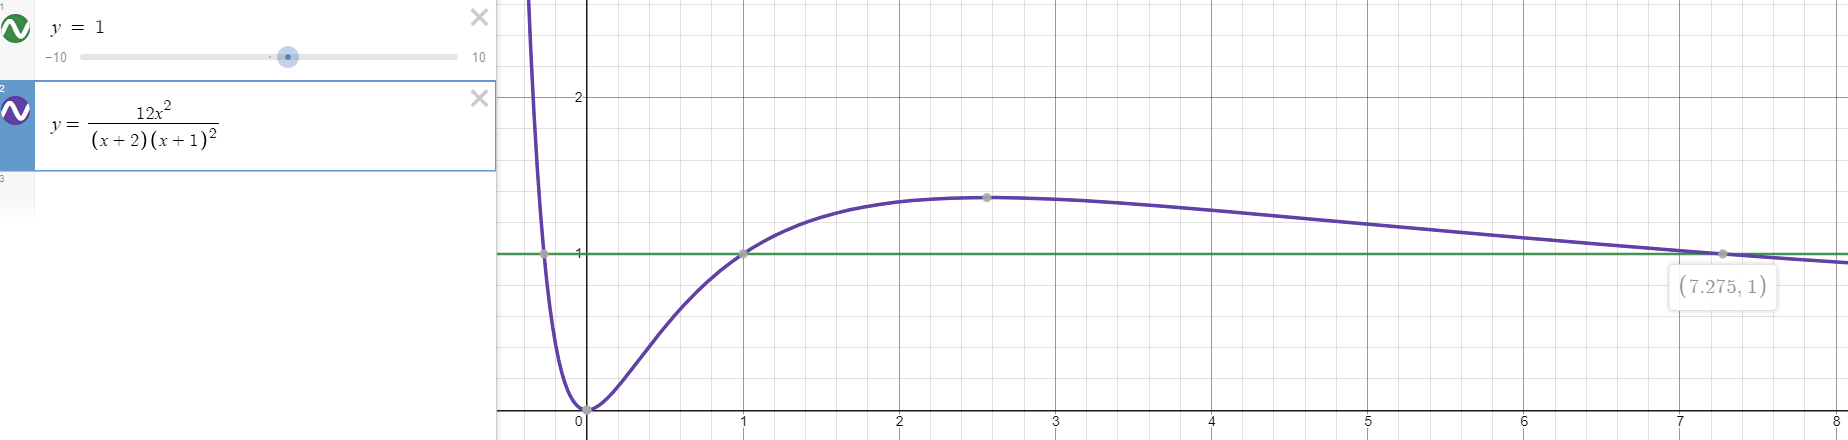
\includegraphics[width=6in]{graph.PNG}
    \end{center}
    The intersection of the graph is at $7.275$ and it can be shown that the efficiency is monotonically decreasing for all $n \geq 3$.
        $$\limn\operatorname{eff}(\that_1,\,\that_2) = \limn \frac{12n^2}{(n+2)(n+1)^2} = 0$$
    Therefore, for $n \in [8, \infty)$, $\that_2$ is a better estimator. Since this covers a wider range of possibilities,  $\that_2$ is generally better.
\end{enumerate}